\documentclass[a4paper,12pt]{article}

\usepackage[german]{babel}
\usepackage[utf8]{inputenc}
\usepackage{color}
\usepackage{graphicx}
\usepackage{fancyhdr}
 \usepackage{babelbib}
\usepackage{longtable}
\usepackage{listings}
\usepackage{hyperref}
\usepackage{pdfpages}
\hypersetup{pdftitle={Java 7 - Stand der Technik}}
\pagestyle{fancy}
\footskip=5em

\lstset{
language=Java,
morekeywords={*,...} % if you want to add more keywords to the set
}

\author{Jonas Traub \& Matthis Hauschild}
\title{Sprachänderungen aus Java 7}

\lhead{}
\chead{Sprachänderungen aus Java 7}
\rhead{\thepage}
\lfoot{}
\cfoot{}
\rfoot{}

\begin{document}
\begin{titlepage}
    \begin{center}
     
\includegraphics[height=2.6cm]{images/dhbw.png}

      \vspace*{12mm}    
      TIAI3117 : Technisch-Wissenschaftliches Arbeiten\\
      \vspace*{30mm}    
      {\Huge{Sprachänderungen aus Java 7}}\\
      \vspace*{5mm}    
      Literaturrecherche $\cdot$ Stand der Technik\\
\vspace*{35mm}

\begin{tabular}{c|c}
Jonas Traub & Matthis Hauschild\\
IBM Deutschland & IBM Deutschland\\
%Duale Hochschule Baden-Württemberg & Duale Hochschule Baden-Württemberg\\
DHBW Stuttgart & DHBW Stuttgart\\
jonas.traub@de.ibm.com & matthis.hauschild@de.ibm.com\\
 & \\
 & \\

\includegraphics[height=1.8cm]{images/OCPJ6P.png} 
\includegraphics[height=1.8cm]{images/OCPJ7P.png} & 
\includegraphics[height=1.8cm]{images/OCPJ6P.png} 
\includegraphics[height=1.8cm]{images/OCPJ7P.png}\\
\end{tabular}

      \vfill
      \vspace*{70mm}
      Stuttgart, \today
    \end{center}
\end{titlepage}


\newpage

\tableofcontents
\newpage
%
\section{Literaturrecherche}
Die folgenden Schritte wurden unternommen: TODO

\subsection{Allgemeines Vorgehen}

Es wurden folgende Schritte unternommen um einen möglichst umfangreichen Überblick über alle verfügbaren Quellen zu erhalten:
\begin{enumerate}
\item TODO
\item TODO
\end{enumerate}
Im folgenden Abschnitt ist eine Übersicht über alle genutzen Ressourcen in tabellarischer Form zu finden. Ab Seite \pageref{startdetails} werden die Ergebnisse und Erfahrungen mit diesen Ressourcen näher vorgestellt.

\subsection{Ressourcenübersicht}

\renewcommand{\arraystretch}{1.5}
\begin{table}[htp]
\centering
\begin{tabular}{p{3.6cm}|p{3.5cm}|l|p{3.5cm}}
Resourcentyp & Resource & Datum & Suchergebnisse\\
\hline
Literaturdatenbank/ Bibliothek & DHBW Bibliothek & 26.02.2013 & 5 nutzbare Ergebnisse\\
Patentdatenbank & Deutsches Patent- und Markenamt & 26.02.2013 & 2476x Java (Titel), 0x Java 7 (Titel), 3521x Java 7 (Volltext), keine nutzbaren Ergebnisse\\
Literaturdatenbank & Association for Computing Machinery & 27.02.2013 & 45637 Treffer, davon 1 vielversprechend.\\
Internetquelle & Google & 27.02.2013 & TODO\\
Internetquelle & Wikipedia & 02.03.2013 & TODO\\
\end{tabular}
\end{table}
\renewcommand{\arraystretch}{1}

\label{startdetails}
\subsection{Bibliothek der DHBW Stuttgart}
Die Hochschulbibliothek der DHBW Stuttgart\footnote{http://www.dhbw-stuttgart.de/themen/service-einrichtungen/bibliothek.html} bietet einen Bibliothekskatalog der online\footnote{http://www.dhbw-stuttgart.de/themen/service-einrichtungen/bibliothek/\\bibliothekskatalog-konto.html} durchsucht werden kann. Es wird eine Volltextsuche verwendet. Eine Suche nach \glqq Java\grqq ~ergab 22 Treffer. Eine Suche nach \glqq Java 7\grqq ~ergab 5 Treffer.

\begin{center}
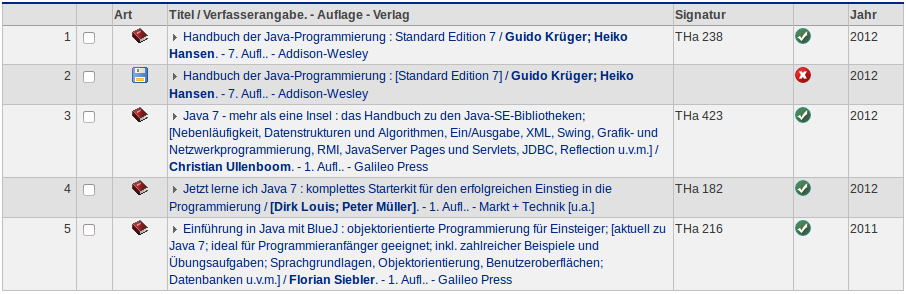
\includegraphics[width=\textwidth]{images/dhbw-lib-search-results.png}
\end{center}

Wir haben alle gelisteten Bücher zu Java 7 vor Ort in der Bibliothek gesichtet. Von den gelisteten Exemplaren ging nur ein Werk\cite{javainsel2} direkt auf die Neuerungen in Java 7 ein. Die anderen Fachbücher stellen eine allgemeine Beschreibungen der Java SE Bibliotheken dar denen lediglich Java in Version 7 zu Grunde liegt\cite{dhLibHandbuchJava} oder Sie richten sich gezielt nur an Javaanfänger\cite{dhLibJetztJavaLernen}\cite{dhLibBlueJStart}, wodurch sie für eine weitere Betrachtung im aktuellen Kontext nicht interessant sind.\\

Das Buch \glqq Java 7 - Mehr als eine Insel\grqq\cite{javainsel2} ~beschreibt in einem eigenen Kapitel die Neuerungen in Java 7. Der Autor, Christian Ullenboom, ist uns bereits durch seine frühere Veröffentlichung \glqq Java ist auch eine Insel\grqq\cite{javainsel1} ~bekannt gewesen, die mittlerweile als Referenzwerk für die Java SE Bibliotheken gehandelt wird. Die aktuelle Ausgabe dieses Buchs basiert ebenfalls auf Java 7 und kann im \glqq Stand der Technik\grqq ~Dokument verwendet werden.

\subsection{DPMA - Deutschel Patent- und Markenamt}
Wir haben die Einsteigersuche\footnote{http://depatisnet.dpma.de/DepatisNet/depatisnet?action=einsteiger} des DPMA verwendet um Patente mit Bezug zum Thema Java 7 zu finden. Eine Suche im Titel ergab hierbei für \glqq Java 7\grqq ~keinen Treffer und für \glqq Java \grqq ~2476 Treffer. In der Volltextsuche wurden für \glqq Java 7\grqq ~3521 Ergebnisse gefunden.\\

Um aktuelle Neuerungen zu finden wurde zusätzlich die Sortierung nach Veröffentlichungsdatum genutzt. Bei unserer Recherche war es in der Menge der Ergebnisse nicht möglich auch nur einen Eintrag aufzufinden, der sich auf Neuerungen in der Sprache bezieht. Alle betrachteten Einträge verwenden lediglich Java. Dar Java SE 7 an sich als Open Source verfügbar ist, ist es generell unwahrscheinlich das Patente auf offizielle Sprachänderungen an Java bestehen.\\

\subsection{ACM - Association for Computing Machinery}
Unter verwendung des Suchbegriff \glqq New Features in Java 7 \grqq ~wurden 45637 Treffer erzielt.
Weitere Suchbegriffe ergaben noch deutlich mehr Treffer.\\

Einige der aufgefundenen Artikel lassen einen Interessanten Inhalt, auch im Bezug auf das Thema dieser Arbeit, vermuten. Leider sind die gefunden Arbeiten in der Regel nur gegen Entgeld erhältlich, wodurch wir für weitere Betrachtungen andere Quellen bevorzugt haben.\\

Der vielversprechendste Treffer ist der Artikel \glqq An introduction to Java development kit 7 \grqq\cite{acmJava7} ~von Daryl Mayer, Nikola Grecevski und Vijay Sundaresan.

\subsection{Search Data Backup}
Eine Suche nach \glqq Java 7 Features\grqq\footnote{http://searchdatabackup.techtarget.com/search/query?q=Java+7+features} ~lieferte sehr viele Ergebnisse mit direktem Bezug zu den aktuellen Sprachänderungen. Aus der vielzahl der guten Ergebnisse musste selektiv ausgewählt werden. Wir haben die jenigen Artikel gewählt, die gezielt neue Features aus Java SE 7 vorstellen. So verblieben sechs Artikel in der Auswahl.\\

Ein Artikel\cite{sbJ7ImproveSec} betrachten den Einfluss neuer Features auf die Sicherheit von Java, ein Artikel\cite{sbJ7literals} beschreibt Änderungen an Literalen, vier Artikel stellen das Automated Resource Management\cite{sbJ7resources}\cite{sbJ7coin} neue Kontrollstrukturen\cite{sbJ7switch} und Supressed Exceptions\cite{sbJ7exeptions} vor.
%
%eof


%
\newpage
\addcontentsline{toc}{section}{Sprachänderungen aus Java 7 - Stand der Technik}
\includepdf{stateofart/stateofart.pdf}
%
\nocite{javainsel2}
\bibliography{stateofart}
\bibliographystyle{gerplain}

\appendix
\section{Verwendete Literatur}

\end{document}
